\chapter{The Coupled Model}
\label{chap:coupledmodel}

\lettrine{N}{umerical} simulations studied by vertex-driven motion and curvature-driven motion as exposed in Chapter~\ref{chap:2dgrains} can be also studied in a coupled way with the purpose of capturing the dynamics of both models and being able to reproduce each one of them individually.
This novel model is called Coupled Model and has been developed in a first version in~\cite{bachelorthesisasazo} and improved during the study of the present Thesis. 
The boundary parametrization proposed here consist in a Lagrange interpolation of $n$ points as follows:
\begin{equation}
    \vxi^{(k)}(s,t) = \boundary,\quad s \in [0,1],
    \label{eq:boundarydiscret}
\end{equation}
where $\phi_i(s)$ are the Lagrange interpolation functions and the points $\x[1]^{(k)}$ and $\x[n]^{(k)}$ are triple junctions. The remaining $n-2$ collocation points are called interior points. For numerical stability each point $\x[i]^{(k)}$ is parametrized on Chebyshev nodes of the second kind~\cite{trefethen2000spectral} using a linear map $[-1,1] \to [0,1]$ to match the definition of $s$.

\section{Derivation of Evolution Equations}

\subsection{Triple Junction Evolution and Normal Component of Interior Points Velocities}
We start with the derivative of the total energy of the grain structure in \eqref{eq:dEdtfull} and we replace the proposed parametrization as:
\begin{equation}
    \frac{dE}{dt}(t) = \int_0^1 -\sum_{k=1}^{K}\left[ \sum_{i=1}^{n} \dotx[i][k](t)  \cdot \int_0^1  \gamma^{(k)}\dTds^{(k)}\!\! \phi_i(s)\,ds \right] + \sum_{m=1}^{M} \vel_m(t) \cdot \sum_{l=1}^3 \gamma^{(m,l)}\T^{(m,l)}.
    \label{eq:dEdtcoupled1}
\end{equation}
In order to find the motion equations of the system we separate the terms related to triple junctions from the summation over grain boundaries in \eqref{eq:dEdtcoupled1} as:
\begin{multline*}
    \frac{dE}{dt}(t) =  -\sum_{k=1}^{K}\left[ \sum_{i=2}^{n-1} \dotx[i][k](t)  \cdot \int_0^1  \gamma^{(k)}\dTds^{(k)}\!\! \phi_i(s)\,ds \right] + \sum_{m=1}^{M} \vel_m(t) \cdot \sum_{l=1}^3 \gamma^{(m,l)}\T^{(m,l)} + \\ \sum_{k=1}^K \left[\dotx[1][k](t)\cdot\int_0^1 \gamma^{(k)} \dTds^{(k)}\!\! \phi_1(s)\,ds + \dotx[n][k](t)\cdot\int_0^1 \gamma^{(k)} \dTds^{(k)}\!\! \phi_n(s)\,ds\right].
\end{multline*}
Then we add them up to the former triple junction term. Notice that we must choose which contribution (from $\x[1][k]$ or $\x[n][k]$) will be added, since for some arbitrary pair of boundaries $\bnd^{(k_1)}, \bnd^{(k_2)}$, the initial and end points coincide, \ie $\x[1][k_1] = \x[n][k_2]$ and we would be adding repeated terms. Re-indexing this contribution in terms of the triple junctions we obtain:
\begin{multline}
    \frac{dE}{dt}(t) =   -\sum_{k=1}^{K}\left[ \sum_{i=2}^{n-1} \dotx[i][k](t)  \cdot \int_0^1  \gamma^{(k)}\dTds^{(k)}\!\! \phi_i(s)\,ds \right] + \sum_{m=1}^{M} \vel_m(t) \cdot \sum_{l=1}^3 \gamma^{(m,l)}\T^{(m,l)}\\ -\sum_{m=1}^{M} \dotx[m]\,\,(t) \cdot \sum_{l=1}^3 \int_0^1 \gamma^{(m,l)} \dTds^{(m,l)}\phi_{1,m}(s)\,ds,
    \label{eq:dEdtcoupled3}
\end{multline}
where $\vel_m = \dotx[m]$.
The triple junctions velocity is defined as:
\begin{align}
     \dotx[m]\,\,(t) = -\lambda\sum_{l=1}^{3}\gamma^{(m,l)} \left[\T^{(m,l)} - \int_0^1 \dTds^{(m,l)}\,\phi_{1,m}(s)\,ds \right],
    \label{eq:triplejunctionsvel}
\end{align}
where $\lambda$ is the mobility parameter associated to triple junctions.

In the case of the interior points we are interested in obtain a curvature driven motion behavior as well as maintain stability for the points. The velocity of interior points $\dotx[i][k](t)$ is defined to have a normal component, obtained from the curvature study in Chapter \ref{chap:closedboundary}, and a tangential component that ensures a correct distribution of the interior points along the boundary as:
\begin{equation}
\dotx[i][k](t) = \alpha_i(t)\,\hatT_i(t) + \beta_i(t)\,\hatN_i(t),
\label{eq:ortho_decomp}
\end{equation}
where $\hatT_i$ and $\hatN_i$ are the tangential and normal components of the velocities and $\alpha_i, \beta_i \in \mathbb{R}$ are coefficients to be determined, $\hatT_i\cdot \hatN_i=0$, and $\|\hatT_i\|=\|\hatN_i\|=1$.
In the case of the normal component $\beta_i(t)\,\hatN_i(t)$ it can be obtained directly from \eqref{eq:dEdtcoupled3} as:
\begin{align}
    \beta_i(t)\,\hatN_i(t) = \dotx[i,\hatN][k](t)  = \frac{\mu\gamma^{(k)}}{\norm{\mylvec(s_i,t)}} \int_0^1 \dTds^{(k)}\!\!\phi_i(s)\,ds 
    \label{eq:interiorpointsvel}
\end{align}
where $\mu$ is the mobility for interior points inherited from boundary motion.

\subsection{Tangential Component of Interior Points Velocities}
\label{sec:tangential_component}
Defining only a normal component for interior points evolution does not ensure the stability of the boundary since these points might coalesce. In order to minimize energy we can add a tangential component of velocity as long as it is orthogonal to \eqref{eq:interiorpointsvel}. Specifically, we can force the interior points to be always equispaced with respect to the total boundary arc length. This has been studied in~\cite{Mikula2001, Barrett2007, Barrett2010} where the following restriction has to be met:
\begin{equation*}
    \dfrac{d}{dt}\left(\dfrac{\norm{\mylvec_i(t)}}{\AL(t)}\right)=0, \quad i\in \{2,3,\dots,n-2\},
\end{equation*}
where $\norm{\mylvec_i(t)}$ denotes the local arc length at collocation point $s_i$ and $\AL(t)$ is the arc length of the boundary under analysis. Without loss of generality we omit the indexation of boundaries from this point and the result applies for all boundaries in the system. Continuing the analysis we obtain the following equation:
%
\begin{align}
    \dfrac{\dfrac{d}{dt}\left(\norm{\mylvec_i(t)}\right)
    \mathcal{L}(t)-
    \dfrac{d}{dt}\left(\AL(t)\right)
    \norm{\mylvec_i(t)} }{\AL^2(t)}&=0,\nonumber\\
    \dfrac{d}{dt}\left(\norm{\mylvec_i(t)}\right)
    \mathcal{L}(t)-
    \dfrac{d}{dt}\left(\AL(t)\right)
    \norm{\mylvec_i(t)} &=0,\nonumber\\
    \dfrac{d}{dt}\left(\norm{\mylvec_i(t)}\right)
    \mathcal{L}(t)&=
    \dfrac{d}{dt}\left(\AL(t)\right)
    \norm{\mylvec_i(t)},\label{eq:alpha_eq}
\end{align}
%
where $\dfrac{d}{dt}\left(\norm{\mylvec_i(t)}\right)=\T_i(t)\cdot\dfrac{d}{dt}\left(\mylvec_i(t)\right)$  and $\dfrac{d}{dt}\left(\AL(t)\right)=\displaystyle{\int_0^1 \T(s,t)\cdot \dfrac{d}{dt}\left(\mylvec(s,t)\right)\,ds}$.
Equation \eqref{eq:alpha_eq} needs to be applied to
each interior point, but before we do that, we need to build each element, obtaining a linear system of equations.

Recalling the definition of the boundary in \eqref{eq:boundarydiscret} we define the following components:
\begin{align*}
    \mylvec(s,t) = \dxids(s,t) &= \sum_{i=1}^{n} \x[i](t) \,\phi_i'(s)\\
    &=  \sum_{i=1}^{n} \y[i](t) \,\phi_i(s).
\end{align*}
Computation of such components is widely explained in~\cite{bachelorthesisasazo}. Now, it is direct to compute the derivative
respect to time of $\mylvec(s,t)$ and it is also
direct to obtain,
%
\begin{align*}
\dfrac{\partial \mylvec}{\partial t}(s,t) 
&= \sum_{i=1}^{n} \doty_{i}(t) \,\phi_i(s),\\
\dfrac{d}{dt}\left(\mylvec_i(t)\right)&=\doty_{i}(t).
\end{align*}
%
Thus, plugging in each component to \eqref{eq:alpha_eq} we obtain,
%
\begin{align*}
    \dfrac{d}{dt}\left(\norm{\mylvec_i(t)}\right)
    \,\mathcal{L}(t)&=
    \dfrac{d}{dt}\left(\AL(t)\right)
    \norm{\mylvec_i(t)} \\
    \T_i(t)\cdot\dfrac{d}{dt}\left(\mylvec_i(t)\right)
    \,\AL(t) &= \int_0^1 \T(s,t)\cdot \dfrac{d}{dt}\left(\mylvec(s,t)\right)\,ds\,
    \norm{\mylvec_i(t)}\\
    \T_i(t)\cdot\doty_{i}(t) \,\AL(t) &=
    \int_0^1 \T(s,t)\cdot \left(\sum_{k=1}^{n} \doty_{k}(t) \,\phi_k(s)\right)\,ds\,
    \norm{\mylvec_i(t)}\\
    \T_i(t)\cdot\doty_{i}(t) \,\AL(t) &=
    \left(\sum_{k=1}^{n} \doty_{k}(t)\cdot \int_0^1 \T(s,t)\, \phi_k(s)\,ds\right)\,
    \norm{\mylvec_i(t)}.
\end{align*}
Moving $\norm{\mylvec_i(t)}$ to the right hand side we obtain,
\begin{equation}
    \T_i(t)\cdot\doty_{i}(t) \dfrac{\AL(t)}{\norm{\mylvec_i(t)}} =
    \sum_{k=1}^{n} \doty_{k}(t)\cdot \underbrace{\int_0^1 \T(s,t)\, \phi_k(s)\,ds}_{\displaystyle \mathbf{w}_k(t)}, \quad i\in{2,\dots,n-1}.
    \label{eq:alpha_eq_base}
\end{equation}
%
Now, it is time to use our orthogonal
decomposition \eqref{eq:ortho_decomp} to
obtain the $\alpha_i(t)$, which is achieved
by the following linear transformation with the differentiation matrix $D$ that allows numerical differentiation at Chebyshev nodes.
\begin{equation}
\begin{pmatrix}
\doty_{1}(t) \\
\doty_{2}(t)\\
\vdots\\
\doty_{i}(t)\\
\vdots\\
\doty_{n-1}(t)\\
\doty_{n}(t)
\end{pmatrix}=D\,
\begin{pmatrix}
\dotx_{1}(t)\\
\beta_2(t)\,\hatN_2(t)+\alpha_2(t)\,\hatT_2(t)\\
\vdots \\
\beta_i(t)\,\hatN_i(t)+\alpha_i(t)\,\hatT_i(t)\\
\vdots \\
\beta_{n-1}(t)\,\hatN_{n-1}(t)+\alpha_{n-1}(t)\,\hatT_{n-1}(t)\\
\dotx_{n}(t)
\end{pmatrix}
\label{eq:y_velocities}
\end{equation}

where the vectors $\doty_{i}(t)$, $\hatN_i(t)$, $\hatT_i(t)$, $\dotx_{1}(t)$ and $\dotx_{n}(t)$ are considered row-vectors. Recall that $\dotx_{1}(t)$ and $\dotx_{n}(t)$ are the triple junctions velocities of the boundary. Thus each component of the system can be written as
\begin{equation*}
\doty_{i}(t)
=D_{i,1}\,\dotx_{1}(t)
+\sum_{j=2}^{n-1}D_{i,j}\,\left(\beta_j(t)\,\hatN_j(t)+\alpha_j(t)\,\hatT_j(t)
\right)+D_{i,n}\,\dotx_{n}(t).
\end{equation*}
%
We now first compute the unknown part and the known part of the left hand side of \eqref{eq:y_velocities}, we omit for now the coefficient $\dfrac{\AL(t)}{\norm{\mylvec_i(t)}}$:
%
\begin{align*}
    \T_i(t)\cdot\doty_{i}(t)  &=
    \T_i(t)\cdot\left(D_{i,1}\,\dotx_{1}(t)
+\sum_{j=2}^{n-1}D_{i,j}\,\left(\beta_j(t)\,\hatN_j(t)+\alpha_j(t)\,\hatT_j(t)
\right)+D_{i,n}\,\dotx_{n}(t)\right)\\
&=
    D_{i,1}\,\T_i(t)\cdot\dotx_{1}(t)
+\sum_{j=2}^{n-1}D_{i,j}\,\left(\beta_j(t)\,\T_i(t)\cdot\hatN_j(t)+\alpha_j(t)\,\T_i(t)\cdot\hatT_j(t)
\right)\\
&\phantom{=}+D_{i,n}\,\T_i(t)\cdot\dotx_{n}(t)\\
&=\sum_{j=2}^{n-1}D_{i,j}\,\alpha_j(t)\,\T_i(t)\cdot\hatT_j(t)\\
&\phantom{=}+\left(D_{i,1}\,\T_i(t)\cdot\dotx_{1}(t)+\sum_{j=2}^{n-1}D_{i,j}\,\beta_j(t)\,\T_i(t)\cdot\hatN_j(t)+D_{i,n}\,\T_i(t)\cdot\dotx_{n}(t)\right).
\end{align*}
%
Similarly for the right-hand-side of \eqref{eq:alpha_eq_base} we obtain
the following for the $k$-th element of the sum,
\begin{align*}
    \doty_{k}(t)\cdot \mathbf{w}_k(t)
    &=D_{k,1}\,\mathbf{w}_k(t)\cdot\dotx_{1}(t)
+\sum_{j=2}^{n-1}D_{k,j}\,\left(\beta_j(t)\,\mathbf{w}_k(t)\cdot\hatN_j(t)+\alpha_j(t)\,\mathbf{w}_k(t)\cdot \hatT_j(t)
\right)\\
    &\phantom{=}+D_{k,n}\,\mathbf{w}_k(t)\cdot\dotx_{n}(t)\\
&= \sum_{j=2}^{n-1}D_{k,j}\,\alpha_j(t)\,\mathbf{w}_k(t)\cdot\hatT_j(t)\\
&\phantom{=}+\left(D_{k,1}\,\mathbf{w}_k(t)\cdot\dotx_{1}(t)+\sum_{j=2}^{n-1}D_{k,j}\,\beta_j(t)\,\mathbf{w}_k(t)\cdot\hatN_j(t)+D_{k,n}\,\mathbf{w}_k(t)\cdot\dotx_{n}(t)\right).
\end{align*}
%
So, collecting the unknown terms on the left hand side 
and the known terms on the right hand side we
finally obtain the linear system of equations we
need to solve to obtain the $\alpha_i(t)$,
%
\begin{align*}
    \dfrac{\AL(t)}{\norm{\mylvec_i(t)}}
    \sum_{j=2}^{n-1}D_{i,j}\,\alpha_j(t)\,\T_i(t)\cdot\hatT_j(t)-\sum_{k=1}^n \sum_{j=2}^{n-1}D_{k,j}\,\alpha_j(t)\,\mathbf{w}_k(t)\cdot\hatT_j(t)=&\\
    -\dfrac{\AL(t)}{\norm{\mylvec_i(t)}}\left(D_{i,1}\,\T_i(t)\cdot\dotx_{1}(t)+\sum_{j=2}^{n-1}D_{i,j}\,\beta_j(t)\,\T_i(t)\cdot\hatN_j(t)+D_{i,n}\,\T_i(t)\cdot\dotx_{n}(t)\right)\\
    +
    \sum_{k=1}^n
    \left(D_{k,1}\,\mathbf{w}_k(t)\cdot\dotx_{1}(t)+\sum_{j=2}^{n-1}D_{k,j}\,\beta_j(t)\,\mathbf{w}_k(t)\cdot\hatN_j(t)+D_{k,n}\,\mathbf{w}_k(t)\cdot\dotx_{n}(t)\right).
\end{align*}
%
Collecting the coefficient that multiply $\alpha_i(t)$ and rearranging the right-hand-side we obtain,
\begin{align*}
    \sum_{j=2}^{n-1}\left(D_{i,j}\dfrac{\AL(t)}{\norm{\mylvec_i(t)}}\,\T_i(t)-\sum_{k=1}^n D_{k,j}\mathbf{w}_k(t)\right)\cdot\hatT_j(t)\,\alpha_j(t)=&\\
    % -\left(D_{i,1}\dfrac{\mathcal{L}(t)}{\norm{\mylvec_i(t)}}\,\T_i(t)-\sum_{k=1}^n D_{k,1}\mathbf{w}_k(t)\right)\cdot\dotx_{1}(t)
    % \\
    % -\sum_{j=2}^{n-1}\left(D_{i,j}\dfrac{\AL(t)}{\norm{\mylvec_i(t)}}\,\T_i(t)-\sum_{k=1}^n (D_{k,j}\,\mathbf{w}_k(t)-D_{i,j}\,\T_i(t))\right)\cdot(\beta_j(t)\,\hatN_j(t))
    % \\
    % -
    % \left(D_{i,n}\dfrac{\mathcal{L}(t)}{\norm{\mylvec_i(t)}}\,\T_i(t)-\sum_{k=1}^n D_{k,n}\mathbf{w}_k(t)\right)\cdot\dotx_{n}(t)
    -\dfrac{\mathcal{L}(t)}{\norm{\mylvec_i(t)}}\left(D_{i,1}\,\dotx_{1}(t)+\sum_{j=2}^{n-1}D_{i,j}\,\beta_j(t)\,\hatN_j(t)+D_{i,n}\,\dotx_{n}(t)\right)\cdot\T_i(t)\\
    +
    \sum_{k=1}^n
    \left(D_{k,1}\,\dotx_{1}(t)+\sum_{j=2}^{n-1}D_{k,j}\,\beta_j(t)\,\hatN_j(t)+D_{k,n}\,\dotx_{n}(t)\right)\cdot\mathbf{w}_k(t).
\end{align*}
%
Thus, we have shown how to obtain the coefficient $\alpha_i(t)$. 
They need to be computed explicitly
every time the interior points will move
or when we need to compute quantities
that depend on their velocity, such as
the extinction time of each grain boundary.


\section{Numerical Implementation}

\subsection{Estimation of Extinction Time}
The extinction time $t_{\text{ext}}$ is defined as the time when a boundary collapses and its arc length becomes zero.
Consider the arc length of a boundary as a function of time $\AL(t)$. 
The arc length at time $t+\Delta t$ can be estimated as
\begin{equation*}
    \AL(t+\Delta t) = \AL(t) + \Delta t\, \AL'(t)+\mathcal{O}((\Delta t)^2).
\end{equation*}
To determine if a boundary is shrinking or not we need to compute $\AL'(t)$. If $\AL'(t)$ is negative it shrinks. If we consider that the boundary collapses within $[t, t+\Delta t]$, \ie $\AL(t+t_{\text{ext}}) = 0$ we can estimate the extinction time as follows:
\begin{align*}
0 &\approx \AL(t) + t_{\text{ext}} \,\AL'(t)\\
t_{\text{ext}} &\approx -\dfrac{\AL(t)}{\AL'(t)}.
\end{align*}
%
An important result of the study of extinction time is that topological transitions are delayed because the extinction time estimation has an error proportional to the simulation time step $\Delta t$. Figure~\ref{fig:coupled_texts} shows extinction times over time for a boundary that has to flip but nevertheless when the extinction time is close to $\Delta t$ the estimation fails and the boundary cannot flip. 
Even if we decrease $\Delta t$ the flipping is delayed. 
This analysis suggests that the continuous motion of triple junctions and boundaries has to be more accurate than estimation of the extinction time.
%
\begin{figure}
    \centering
    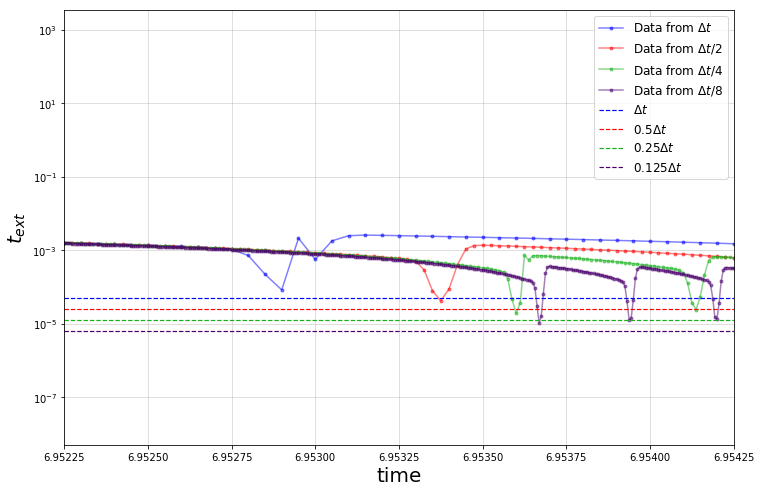
\includegraphics[width=12cm]{figures/coupled/image_preview.png}
    \caption[Example of delayed flipping.]{Example of a delayed flipping. The extinction time being proportional to the simulation $\Delta t$ (dashed lines) is computed with proportional error and flippings are delayed or never detected.}
    \label{fig:coupled_texts}
\end{figure}
%
The first idea to obtain a better approximation of extinction time is to perform $r$ steps of size $\Delta \tau$ such that $r \Delta \tau = \Delta t$. During the execution of this steps, the basic assumption is that no topological transition occurs and thus the system just evolves. Using a smaller time step helps to ensure a better approximation. On the other hand, straightforward higher order methods can be used. For example second order Runge-Kutta ensures that the grain system evolves with precision $\mathcal{O}(\Delta t^2)$, and therefore the extinction time has the same precision. Runge-Kutta can also be improved by the introduction of many steps of smaller size. Both methods must detect the upcoming topological transitions and after the evolution is complete the transitions are handled.

%In both methods, topological transitions that might occur in $[t, t+\Delta t]$ are detected and managed after the evolution is performed. Both methods are discussed below.

\subsection{Multistep Euler}

This method assumes that Euler method can be improved if steps of smaller size are performed to evolve the grain structure previous to handle topological transitions. A number $r$ of smaller steps of size $\Delta \tau$ is chosen, where $\Delta \tau = \Delta t / r$. The execution of this $r$ steps is called the \emph{multistep stage} and the system evolves assuming that there are not topological transitions. Algorithm~\ref{alg:multistep} shows this method.

\begin{algorithm}
\caption{Multistep Euler for Coupled Model}
\label{alg:multistep}
\begin{algorithmic}[1]
\Procedure{ME}{}
\State $\Delta \tau \gets \dfrac{\Delta t}{r}$ Time step of multistep phase.
\For{$k:1,\dotso,r$}
%\State Detect Topological Transitions
\State $\mathbf{V}_t \gets$ Compute velocities
\State $\vertices_{t + \Delta \tau} \gets \vertices_{t} + \Delta \tau \mathbf{V}_t$
\State $t \gets t + \Delta \tau$
\EndFor
\EndProcedure
\end{algorithmic}
\end{algorithm}

Using a smaller step-size helps to ensure a better approximation of the extinction time proportional to $\mathcal{O}(\Delta \tau)$.

%Inside the multistep stage, topological transitions are detected by computing the extinction time of the boundaries and comparing it with $\Delta t$ but they are not performed. When the multistep stage is over all the topological transitions found are filtered so there are no inconsistencies and then are performed safely.

No extra memory is required for this method, but the cost is purely computational since the method is performing $r$ steps per main step and thus is almost $r$ times slower.  
Notice that when $r = 1$, we recover the original Forward Euler method.

\subsection{Multistep Second Order Runge-Kutta}

If the goal is to obtain a good approximation of the extinction time, a higher order method can be implemented straightforward. For example extinction times with precision $\mathcal{O}(\Delta t^2)$ can be estimated using second order Runge-Kutta (RK2). We can also improve this method by means of introducing the multistep idea to perform several RK2 steps within $[t,t+\Delta t]$ as shown in Algorithm~\ref{alg:rk2}.

\begin{algorithm}
\caption{Multistep Second Order Runge-Kutta for Coupled Model}
\label{alg:rk2}
\begin{algorithmic}[1]
\Procedure{MRK2}{}
\State $\Delta \tau \gets \dfrac{\Delta t}{r}$ Time step of multistep phase.
\For{$k:1,\dotso,r$}
\State $\mathbf{\overline{\vertices}}_t \gets$ Backup positions $\vertices_t$ of triple junctions and interior points
\State $\mathbf{V}_t \gets$ Compute velocities
\State $\vertices_{t + \Delta \tau / 2} \gets \vertices_t + \dfrac{\Delta \tau}{2} \mathbf{V}_t$. Evolve structure for first RK estimation
\State $\mathbf{V}_{t + \Delta \tau /2} \gets$ Compute velocities
\State $\vertices_{t + \Delta \tau} \gets \mathbf{\overline{\vertices}}_t + \Delta \tau \mathbf{V}_{t + \Delta \tau /2}$ . Evolve structure for second RK estimation
\State $t \gets t + \Delta \tau$
\EndFor
\EndProcedure
\end{algorithmic}
\end{algorithm}

The cost of this method lies in the memory needed to store the extra data for performing the two estimations at time $\Delta \tau/2$ and $\Delta \tau$ and the number of steps $r$. Notice that when $r = 1$  we recover the original RK2. In this implementation it is only necessary to backup the positions of the vertices and interior points to be used in the last step of the method and not the whole data structure \ie arc lengths, curvatures, grain areas, etc.

\subsection{Extinction Time Estimation with Multistep Methods}

Given the proposed multistep methods to evolve the grain network, a final step is required in the analysis. The question here is: What is the correct interval that we should look detect upcoming flippings? When we start a time simulation $t$, we need to detect all topological transitions that, once they are resolved, we can start the next step $t+\Delta t$ safely.

We should first look ahead for all events between $[0, 2\Delta t]$, since those events have to be checked before advance to $\Delta t$, otherwise we might be losing them and delaying them unnecessarily. The next step, which is an inner step $t+\Delta \tau$ only needs to check the extinction times in $[0, 2\Delta t - \Delta \tau]$ since we just advanced $\tau$. Notice that we are just detecting and not performing the flippings. 
We continue this methodology along the $r$ steps. Before passing to the next time $t+\Delta t$ we collect the flippings and perform only those which will not introduce race conditions, \ie flippings that will not modify the same neighborhood of vertices and boundaries. 
This is addressed in Chapter~\ref{chap:parallelflip}. 
After the topological transitions are solved, we are ready to start with a safe structure at time $t+\Delta t$. 
Figure~\ref{fig:coupled_deltat} shows an sketch of the detection algorithm used with the multistep algorithms.

\begin{figure}[t]
    \centering
    \begin{tikzpicture}
        % coordinates
        \coordinate (x0) at (-1,0);
        \coordinate (x1) at (0,0);
        \coordinate (x2) at (1.5,0);
        \coordinate (x3) at (3,0);
        \coordinate (x4) at (4.5,0);
        \coordinate (x5) at (6,0);
        \coordinate (x6) at (12,0);
        \coordinate (x7) at (13,0);
        \coordinate (A) at (4.2,2);
        
        % vertices
        \filldraw [black] (x1) circle (1.5pt);
        \filldraw [black] (x2) circle (1.5pt);
        %\filldraw [black] (x3) circle (1.5pt);
        \filldraw [black] (x4) circle (1.5pt);
        \filldraw [black] (x5) circle (1.5pt);
        \filldraw [black] (x6) circle (1.5pt);
        
        %%%%%%%%%%%%%%%%%%%%%%%%%%%%%%%%%%%%%%%%%%%%%
        % boundaries
        \draw[line width=0.4mm, black] (x1) -- (x6);
        \draw[line width=0.4mm, black, dashed] (x0) -- (x1);
        \draw[line width=0.4mm, black, dashed] (x6) -- (x7);
        
        \draw[decoration={calligraphic brace,mirror,amplitude=1em,raise=1.5em},decorate,line width=1.5pt, pen colour={Red}]
          (x1) -- node[below=2.5em, color=Red,text width=4cm] {\textsf{Detect flippings with} $t_{\text{ext}} \in [0, 2\Delta t- r\Delta \tau]$} (x6);
         
        \node[shape=circle,draw,inner sep=1pt,line width=1pt, color=Red] at (3.6,-1.4) {\textsf{1}};
         
        \node[shape=circle,draw,inner sep=1pt,line width=1pt, color=Green] at (6.1,0.77) {\textsf{3}};
         
        \draw[pen colour={Green}, decoration={calligraphic brace,amplitude=1em,raise=0.3em},decorate,line width=1.5pt]
          (x5) -- node[above=1em,color=Green,text width=5cm] {\textsf{Advance to this zone safely}} (x6);
         
         
         \node[shape=circle,draw,inner sep=1pt,line width=1pt, color=Orange] at (1.6,2.8) {\textsf{2}};
         
         \draw[->,Orange,ultra thick] (A) -- ($(x5)+(-0.1,0.1)$);
         \node[draw=none, color=Orange, above, text width=4.5cm] at (A) {\textsf{Perform flippings before advance to} $t+\Delta t$};
        
        % Text
        \node[draw=none, color=black, below] at (x1) {$t$};
        \node[draw=none, color=black, below] at (x2) {$\scriptstyle t+\Delta \tau$};
        \node[draw=none, color=black, below] at (x3) {$\phantom{a}\ldots\phantom{a}$};
        %{$\scriptstyle t+2\Delta \tau$};
        \node[draw=none, color=black, below] at (x4) {$\scriptstyle t+(r-1)\Delta \tau$};
        \node[draw=none, color=black, below] at (x5) {$t+\Delta  t$};
        \node[draw=none, color=black, below] at (x6) {$t+2\Delta  t$};
    \end{tikzpicture}
    \caption{Flipping detection mechanism that prevents delay in topological transitions.}
    \label{fig:coupled_deltat}
\end{figure}

\subsection{Predictor-Corrector Algorithm}

The tangential component $\hatT_i$ of the total velocity of interior points, explained in Section~\ref{sec:tangential_component}, helps to avoid the interior points coalescing and its computation depends partially on the normal component $\displaystyle \beta_i(t)\,\hatN_i$. 
When the boundaries are shrinking and close to collapse, the curvature of the boundary grows a lot and thus the vector $\beta_i(t)\,\hatN_i$ is large, requiring a very small $\Delta t$ to perform a stable evolution. 
The computation of $\hatT_i$ depends on $\beta_i(t)\,\hatN_i$ and thus also grows. %the computation of $\hatN_i$ becomes unstable and therefore the computation of $\hatT_i$ too, 
The magnitude of these vectors increases and leads to unstable boundaries with irregular shapes and delayed flippings since the unstable boundaries actually grew and may present negative extinction times, (\ie the boundary grows) or large positive extinction times (the boundary will collapse in a time greater than $\Delta t$). 
Thus we must be able to detect when this behavior will happen prior to the boundary collapse without assuming anything about the boundary shape and just looking to the total velocities.
%
\begin{figure}[ht]
    \centering
    \subfloat[Sketch of a boundary with two interior points marked in blue. 
    The \emph{candidate} steady state is marked in red on the dashed gray line.
    The location of the interior points on the next time-step shall not cross the \emph{candidate} steady state in red.]{
    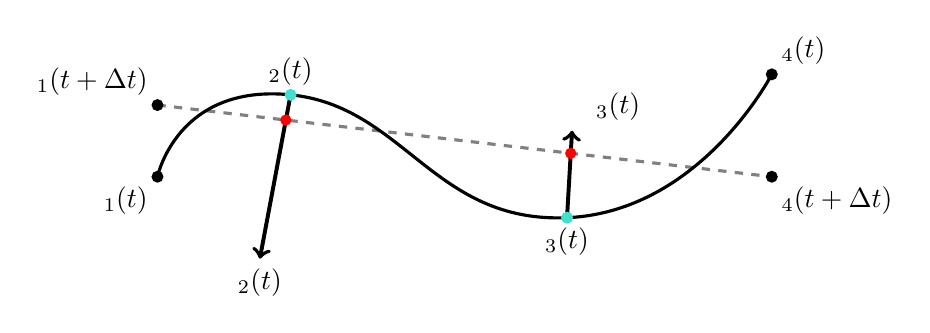
\begin{tikzpicture}[scale=1.3]
        % Vertices at time t
        \coordinate (x0) at (0,0);
        \coordinate (x1) at (6,1);
        % interior points at time t
        \coordinate (i0) at (1.3,0.8);
        \coordinate (i1) at (4,-0.4);
        % Vertices at time t+dt
        \coordinate (x2) at (0,0.7);
        \coordinate (x3) at (6,0);
        % interior points at time t+dt
        %\coordinate (i2) at (0.25, 4.5);
        %\coordinate (i3) at (4,-0.4);

        % Labels
        \node[draw=none, color=black, above left] at (x2) {$\x_1(t+\Delta t)$};
        \node[draw=none, color=black, below right] at (x3) {$\x_4(t+\Delta t)$};
        \node[draw=none, color=black, below left] at (x0) {$\x_1(t)$};
        \node[draw=none, color=black, above right] at (x1) {$\x_4(t)$};
        \node[draw=none, color=black, above] at (i0) {$\x_2(t)$};
        \node[draw=none, color=black, below] at (i1) {$\x_3(t)$};
        
        \node[draw=none, color=black, below] at (1,-0.8) {$\dotx_2(t)$};
        \node[draw=none, color=black, above] at (4.5,0.45) {$\dotx_3(t)$};
        % Vertices have evolved and we mark de future steady state
         \draw[line width=0.4mm, black!50, dashed] (x2) -- (x3);
        % Draw the boundary as seen by the interior points which have not been moved
        \draw[line width=0.4mm] plot [smooth, tension=1] coordinates {(x0) (i0) (i1) (x1)};
        
        % Draw velocities
        \draw[->,black,line width=0.5mm] (i0) -- (1,-0.8);
        %\draw[->,black,line width=0.5mm] (i1) -- (4.1,1.3);
        \draw[->,black,line width=0.5mm] (i1) -- (4.05,0.45);
        
        % Draw vertices
        \filldraw [black] (x0) circle (1.5pt);
        \filldraw [black] (x1) circle (1.5pt);
        \filldraw [black] (x2) circle (1.5pt);
        \filldraw [black] (x3) circle (1.5pt);
        % Draw inner points
        \filldraw [Turquoise] (i0) circle (1.5pt);
        \filldraw [Turquoise] (i1) circle (1.5pt);
        %\filldraw [red] (i2) circle (1.5pt);
        %\filldraw [red] (i3) circle (1.5pt);
        \filldraw [red] (1.25382, 0.55372) circle (1.4pt);
        \filldraw [red] (4.037, 0.229015) circle (1.4pt);
    \end{tikzpicture}
    \label{fig:predcorr1}
    }\\
    \subfloat[The prediction stage. 
    Interior points predict their 
    location at next time-step, marked in blue, given the current total velocities. 
    %They might or not cross the future \emph{candidate} steady state in dashed gray line.
    ]{
        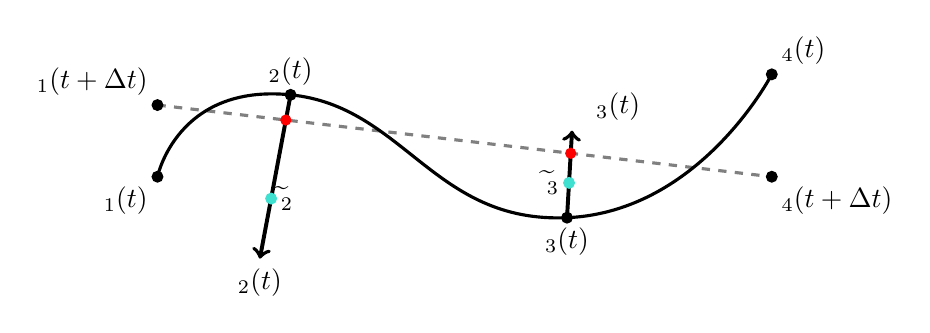
\begin{tikzpicture}[scale=1.3]
        % Vertices at time t
        \coordinate (x0) at (0,0);
        \coordinate (x1) at (6,1);
        % interior points at time t
        \coordinate (i0) at (1.3,0.8);
        \coordinate (i1) at (4,-0.4);
        % Vertices at time t+dt
        \coordinate (x2) at (0,0.7);
        \coordinate (x3) at (6,0);
        % interior points at time t+dt
        %\coordinate (i2) at (0.25, 4.5);
        %\coordinate (i3) at (4,-0.4);

        % Labels
        \node[draw=none, color=black, above left] at (x2) {$\x_1(t+\Delta t)$};
        \node[draw=none, color=black, below right] at (x3) {$\x_4(t+\Delta t)$};
        \node[draw=none, color=black, below left] at (x0) {$\x_1(t)$};
        \node[draw=none, color=black, above right] at (x1) {$\x_4(t)$};
        \node[draw=none, color=black, above] at (i0) {$\x_2(t)$};
        \node[draw=none, color=black, below] at (i1) {$\x_3(t)$};
        
        \node[draw=none, color=black, below] at (1,-0.8) {$\dotx_2(t)$};
        \node[draw=none, color=black, above] at (4.5,0.45) {$\dotx_3(t)$};
        % Vertices have evolved and we mark de future steady state
         \draw[line width=0.4mm, black!50, dashed] (x2) -- (x3);
        % Draw the boundary as seen by the interior points which have not been moved
        \draw[line width=0.4mm] plot [smooth, tension=1] coordinates {(x0) (i0) (i1) (x1)};
        
        % Draw velocities
        \draw[->,black,line width=0.5mm] (i0) -- (1,-0.8);
        %\draw[->,black,line width=0.5mm] (i1) -- (4.1,1.3);
        \draw[->,black,line width=0.5mm] (i1) -- (4.05,0.45);
        
        % Draw vertices
        \filldraw [black] (x0) circle (1.5pt);
        \filldraw [black] (x1) circle (1.5pt);
        \filldraw [black] (x2) circle (1.5pt);
        \filldraw [black] (x3) circle (1.5pt);
        % Draw inner points
        \filldraw [black] (i0) circle (1.5pt);
        \filldraw [black] (i1) circle (1.5pt);

        \coordinate (pred1) at (1.11, -0.213333);
        \coordinate (pred2) at (4.02,-0.06);
        % Draw predictions
        \filldraw [Turquoise] (pred1) circle (1.5pt);
        \filldraw [Turquoise] (pred2) circle (1.5pt);

        \node[draw=none, color=black, right] at (pred1) {$\widetilde{\x}_2$};
        \node[draw=none, color=black, left] at (pred2) {$\widetilde{\x}_3$};

        \filldraw [red] (1.25382, 0.55372) circle (1.4pt);
        \filldraw [red] (4.037, 0.229015) circle (1.4pt);
    \end{tikzpicture}
    \label{fig:predcorr2}
    }\\
    \subfloat[The interior point velocities
    are corrected such that their location at next time-step, marked in blue, is at most the \emph{candidate} steady state locations from Figure \ref{fig:predcorr2} in red.  
    The correction here corresponds to modify the velocity $\dotx_2(t)$ to $\widetilde{\dotx}_2(t)$ as indicated in Algorithm~\ref{alg:predcorr}. 
    The velocity $\dotx_3(t)$ remains the same.]{
        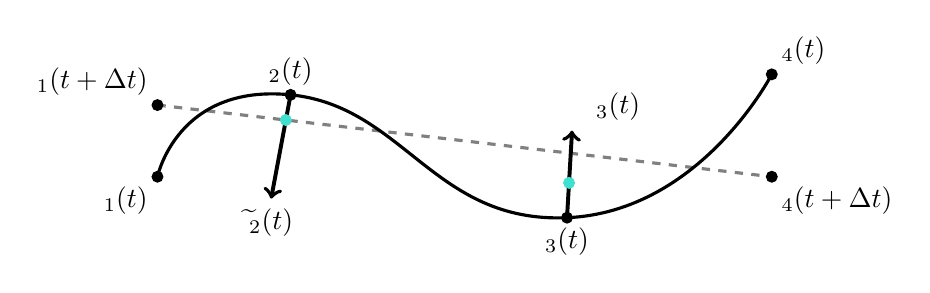
\begin{tikzpicture}[scale=1.3]
        % Vertices at time t
        \coordinate (x0) at (0,0);
        \coordinate (x1) at (6,1);
        % interior points at time t
        \coordinate (i0) at (1.3,0.8);
        \coordinate (i1) at (4,-0.4);
        % Vertices at time t+dt
        \coordinate (x2) at (0,0.7);
        \coordinate (x3) at (6,0);
        \coordinate (pred1) at (1.25382, 0.55372);
        \coordinate (pred2) at (4.02,-0.06);
        % Labels
        \node[draw=none, color=black, above left] at (x2) {$\x_1(t+\Delta t)$};
        \node[draw=none, color=black, below right] at (x3) {$\x_4(t+\Delta t)$};
        \node[draw=none, color=black, below left] at (x0) {$\x_1(t)$};
        \node[draw=none, color=black, above right] at (x1) {$\x_4(t)$};
        \node[draw=none, color=black, above] at (i0) {$\x_2(t)$};
        \node[draw=none, color=black, below] at (i1) {$\x_3(t)$};
        
        \coordinate (endvel) at (1.11, -0.21333);
        \node[draw=none, color=black, below] at (endvel) {$\widetilde{\dotx}_2(t)$};
        \node[draw=none, color=black, above] at (4.5,0.45) {$\dotx_3(t)$};
        
        % Vertices have evolved and we mark de future steady state
         \draw[line width=0.4mm, black!50, dashed] (x2) -- (x3);
        % Draw the boundary as seen by the interior points which have not been moved
        \draw[line width=0.4mm] plot [smooth, tension=1] coordinates {(x0) (i0) (i1) (x1)};
        
        % Draw velocities
        %\draw[->,black,line width=0.5mm] (i0) -- (1,-0.8);
        \draw[->,black,line width=0.5mm] (i0) -- (endvel);
        \draw[->,black,line width=0.5mm] (i1) -- (4.05,0.45);
        
        % Draw vertices
        \filldraw [black] (x0) circle (1.5pt);
        \filldraw [black] (x1) circle (1.5pt);
        \filldraw [black] (x2) circle (1.5pt);
        \filldraw [black] (x3) circle (1.5pt);
        % Draw inner points
        \filldraw [black] (i0) circle (1.5pt);
        \filldraw [black] (i1) circle (1.5pt);


        % Draw predictions
        \filldraw [Turquoise] (pred1) circle (1.5pt);
        \filldraw [Turquoise] (pred2) circle (1.5pt);

        %\node[draw=none, color=black, right] at (pred1) {$\widetilde{\x}_2$};
        %\node[draw=none, color=black, left] at (pred2) {$\widetilde{\x}_3$};
    \end{tikzpicture}
    \label{fig:predcorr3}
    }\\
    \subfloat[The correction stage. 
    Interior points are moved with corrections, if apply. At this moment the boundary points are safe at $t+\Delta t$.]{
        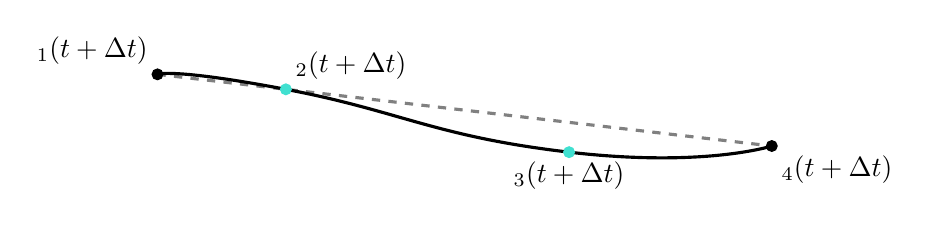
\begin{tikzpicture}[scale=1.3]
        % Vertices at time t
        %\coordinate (x0) at (0,0);
        %\coordinate (x1) at (6,1);
        % Vertices at time t+dt
        \coordinate (x2) at (0,0.7);
        \coordinate (x3) at (6,0);
        
        \coordinate (pred1) at (1.25382, 0.55372);
        \coordinate (pred2) at (4.02,-0.06);
        

        % Labels
        \node[draw=none, color=black, above left] at (x2) {$\x_1(t+\Delta t)$};
        \node[draw=none, color=black, below right] at (x3) {$\x_4(t+\Delta t)$};
        %\node[draw=none, color=black, below left] at (x0) {$\x_1(t)$};
        %\node[draw=none, color=black, above right] at (x1) {$\x_4(t)$};
        \node[draw=none, color=black, above right] at (pred1) {$\x_2(t+\Delta t)$};
        \node[draw=none, color=black, below] at (pred2) {$\x_3(t+\Delta t)$};
        
        % Vertices have evolved and we mark de future steady state
         \draw[line width=0.4mm, black!50, dashed] (x2) -- (x3);
        % Draw the boundary as seen by the interior points which have not been moved
        \draw[line width=0.4mm] plot [smooth, tension=1] coordinates {(x2) (pred1) (pred2) (x3)};
        
        % Draw vertices
        %\filldraw [black] (x0) circle (1.5pt);
        %\filldraw [black] (x1) circle (1.5pt);
        \filldraw [black] (x2) circle (1.5pt);
        \filldraw [black] (x3) circle (1.5pt);
        
        % Draw predictions
        \filldraw [Turquoise] (pred1) circle (1.5pt);
        \filldraw [Turquoise] (pred2) circle (1.5pt);
    \end{tikzpicture}
    \label{fig:predcorr4}
    }
    \caption{Sketch of the Predictor-Corrector Algorithm.}
    \label{fig:predcorr_stages}
\end{figure}

Considering the sketch in Figure~\ref{fig:predcorr1}, which shows a boundary with two interior points $\x_2(t), \x_3(t)$. 
Each interior point has their velocities $\dotx_2(t), \dotx_3(t)$, respectively. 
We evolve the triple junctions given their current velocities and now they move to the locations $\x_1(t+\Delta t)$ and $\x_4(t+\Delta t)$. 
With this information we want to predict where the interior points will be at time $t+\Delta t$.

The prediction stage of the algorithm considers the movement of the interior points using the current velocities, this position $\widetilde{\x}_i$ is called the \emph{prediction}:
%
\begin{equation}
    \widetilde{\x}_i = \x_i(t) + \Delta t\,\dotx_i(t).
\end{equation}
%
Figure~\ref{fig:predcorr2} shows the predictions made for the interior points. Interior point $\x_2(t)$ will be far from the steady state whilst interior point $\x_3(t)$ will be located before the displacement limit.

The correction stage of the algorithm now has to check the following cases given the predictions of the prior stage:
\begin{itemize}
    \item The prediction is beyond the steady state. 
    Since moving to that position generates instability in the boundary and given the fact that we know the steady state line, we set the interior point to evolve at the intersection of the displacement and the steady state. For example, interior point $\x_2$ shall move back to the position in red over the line given by its velocity vector.
    \item The prediction is between the steady state and the current location of the interior point position, so
    we let the point evolve to that position. 
    For example, interior point $\x_3$ can safely evolve to the prediction located at $\widetilde{\x}_3$.
    \item The prediction is before the steady state and before the interior point position.
    This case indicates that for some reason the point is moving away from the steady state and we force the velocity to be zero in order to stop any threat to the stability of the computation.
\end{itemize}
The cases can be algebraically analyzed since we are interested in finding for each interior point the intersections of two straight lines, one line formed by the two vertices at $t+\Delta t$ parametrized by $\omega$, and the other line formed by the interior point at time $t$ and its respective velocity vector at time $t$. Each of this $n-2$ lines can be parametrized by $\omega_i,\; i=2,\ldots,n-1$. The intersection can be written as
%
\begin{equation}
    \x_i + \omega_i\,\dotx_i=
    (1-\omega)\,\x_1 + \omega\, \x_n \label{eq:coupled_lines}
\end{equation}
%
We write \eqref{eq:coupled_lines} as the following system of linear equations:
%For a given interior point $\x_i,\; i=1,\ldots,n-1$

%the intercepts for each line can be solved by the following system:
\begin{equation*}
    \underbrace{\begin{pmatrix}
    \dotx_i \;|\; \x_1 - \x_n
    \end{pmatrix}}_{\displaystyle M} \bm{\omega}_i = \underbrace{\begin{pmatrix}
    \x_1 - \x_i
    \end{pmatrix}}_{\displaystyle \mathbf{b}},
\end{equation*}
where $\bm{\omega}_i = (\omega_i, \omega)^T$ is the intercept vector for each pair of lines. 
Since we need to move along the line given by the velocity of the interior point, we are interested in the first element of $\bm{\omega}_i$ which is $\omega_i$.
Notice that $\omega_i$ is a displacement, and thus it is divided by $\Delta t$. The velocity $\widetilde{\dotx}_i(t)$ is what we call the \emph{correction}.

Figure~\ref{fig:predcorr3} shows the corrections made to the interior points velocities. The velocity $\dotx_2(t)$ had to be scaled by $\omega_2 / \Delta t$ such that the displacement of $\x_2(t)$ is on the steady state limit, that is
\begin{equation*}
\widetilde{\dotx}_2(t) = \frac{\omega_2}{\Delta t}\,\dotx_2(t).     
\end{equation*}
The velocity $\dotx_3(t)$ remains the same since the interior point prediction does not cross the steady state.

Figure~\ref{fig:predcorr4} shows the applied corrections to the interior points movement. Notice that $\x_2$ was moved to the displacement limit whilst $\x_3$ moved without correction.

Algorithm \ref{alg:predcorr} summarizes the predictor-corrector algorithm that has to be applied to each boundary. 
We need to solve the system safely, thus we first check if the system can be solved by checking the determinant of the system matrix $M$ is different from zero given certain tolerance $TOL$. 
The cases when $M$ is singular can be analyzed by looking at its columns. 
If the total velocity of an interior point is $\mathbf{0}$, the first column of $M$ will be null.
If the triple junctions are numerically in the same location we will have the second column of $M$ to be null. 
We set the tolerance $TOL$ to $10^{-12}$. Finally, $M$ will be a singular matrix if the velocity is parallel to the steady state line. In all of these cases there is no need for a correction.

We also need to check a valid value for $\omega_i$. If $\omega_i > 1$ we know that the interior point will not pass over the steady state and we do not apply any correction. 
If $0 < \omega_i < 1$ we need to apply a correction proportional to $\omega_i$. 
Here we are interested in update the velocity of the interior point and thus we divide $\omega_i$ by $\Delta t$. 
If $\omega_i < 0$ the interior point is moving away from the steady state and we set the velocity of the boundary to zero to avoid that point to escape from the steady state.

\begin{algorithm}[t]
\caption{Predictor-Corrector}
\label{alg:predcorr}
\begin{algorithmic}[1]
\Procedure{Pred-Corr}{boundary $\bnd$, $TOL$}
%\State $\bnd \gets$ Boundary to be corrected
% \State $\x_1 \gets$ First vertex of $\bnd$
% \State $\x_2 \gets$ Last vertex of $\bnd$
\State $(\x_1,\x_n) \gets$ First and Last vertex of $\bnd$
\For{$i=2,\ldots,n-1$}
% \State $\x_i \gets $ $i$-th interior point
% \State $\dotx_i \gets$ $i$-th interior point
% velocity 
\State $(\x_i, \dotx_i) \gets $ $i$-th interior point and its total velocity
\State $M \gets \text{GetSystemMatrix}(\x_1, \x_n, \dotx_i)$ \Comment{Notice it is always a $2\times 2$ matrix.}
\If{$|\det(M)| > TOL$}
    \State $\mathbf{b} \gets \x_1 - \x_i$
    \State $\bm{\omega}_i \gets$ \text{Solve} $M \bm{\omega}_i = \mathbf{b}$
    \State $\omega_i \gets $ First component of $\bm{\omega}_i$.
    %\Comment{\textbf{Get }}
    \State $\omega_i \gets \omega_i / \Delta t$
    \If{$\omega_i < 1$}
        \If{$\omega_i > 0$}
            \State $\dotx_i \gets \omega \,\dotx_i$
        \Else
            \State $\dotx_i \gets \mathbf{0}$
        \EndIf
    \EndIf
\EndIf
\EndFor
\EndProcedure
\end{algorithmic}
\end{algorithm}


\section{Numerical Experiments}

The Coupled Model defines several parameters such as the number of interior points $n$, triple junctions mobility $\lambda$, interior points mobility $\mu$, the number of steps for the multistep algorithms $r$ and the step size $\Delta t$. With the introduction of the total velocity of interior points as a combination of a normal component and a tangential component, it is important to maintain the energy decreasing behavior of the simulation. Figure~\ref{fig:coupled_energy} shows the total energy of a simulation of initial \numprint{1000} grains with parameters $\mu=10^{-2}, \lambda=1$ and two interior points. following the energy definition in \eqref{eq:energy}. The behavior despite adding a new component to the velocities remains monotonically decreasing.

\begin{figure}[t]
    \centering
    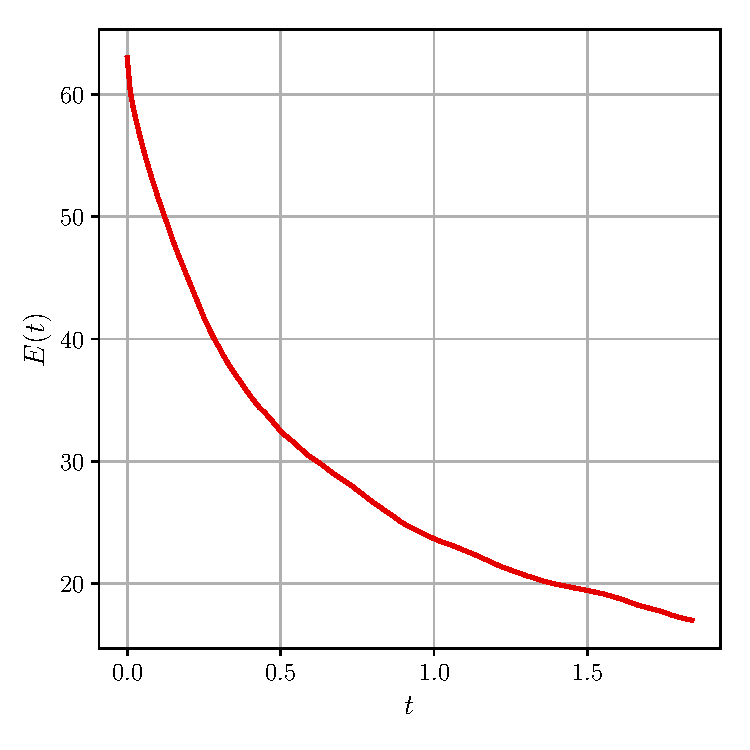
\includegraphics[scale=0.5]{figures/coupled/coupled_model_energy.pdf}
    \caption{Total energy of the grain network with the Coupled Model.}
    \label{fig:coupled_energy}
\end{figure}


\subsection{Statistics}
All experiments were run with initial \numprint{100000} grains, using Euler Multistep with $r=4$, $n=2$ interior points. Figure~\ref{fig:coupled_1} shows the statistics for a simulation with parameters $\mu = 10^{-3}, \lambda=1$ y $\varepsilon=2\cdot10^{-1}$. 

Distribution of relative areas is shown in Figure~\ref{fig:coupled_1_areas}. Experimental data is shown in red. The algorithm managed to remove small grains and reached a distribution which resembles a log-normal, but we still watch the effect of remaining small grains.

Figure~\ref{fig:coupled_1_dihedral} shows the dihedral angle distribution in blue. Experimental data is shown in colors. which concentrates as expected near the stationary angle of the Herring condition $2\pi/3$. The dispersion may be explained by the fact that we are not running a curvature model alone, \ie we have other velocities components, and the fact that we induced anisotropy by the introduction of grain orientations which may perturb the steady state of triple junctions.

Figure~\ref{fig:coupled_1_gbcd} shows the grain boundary character distribution in red and the energy function in blue. The GBCD is effectively recovered, reaching the minima at $\pm \pi/4$ and maximum at $0$, which are the maxima and minimum respectively of the grain boundary energy function described in \eqref{eq:gamma} which we recall here:
\begin{equation*}
    \gamma^{(k)}(\Delta \alpha) = 1 + \frac{\varepsilon}{2}\left(1-\cos^3(4\Delta\alpha)\right).
\end{equation*}
Figure \ref{fig:coupled_1_nsides} shows the histogram of grains per number of sides. 
The mode of the distribution is in six, which agrees with experimental data. 
There are few big grains but also there are few small grains, specifically three sided grains, which is the effect observed also in relative area distribution.

Figure~\ref{fig:coupled_1_avg} shows the average number of sides of neighbors. 
We observe that grains with fewer sides are surrounded in general by grains with larger number of sides.

Figure~\ref{fig:coupled_1_dadt} shows the area rate of change. 
We observe a linear tendency which is predicted by the $n-6$ Von Neumann-Mullins relation. 
For example six sided grains have their rate of change near zero, grain with less sides tend to shrink and grains with more than six sides grow.


%%% Something like curvature code
\begin{figure}[ht]
    \centering
    \subfloat[Distribution of relative areas in log scale and linear scale.]{
    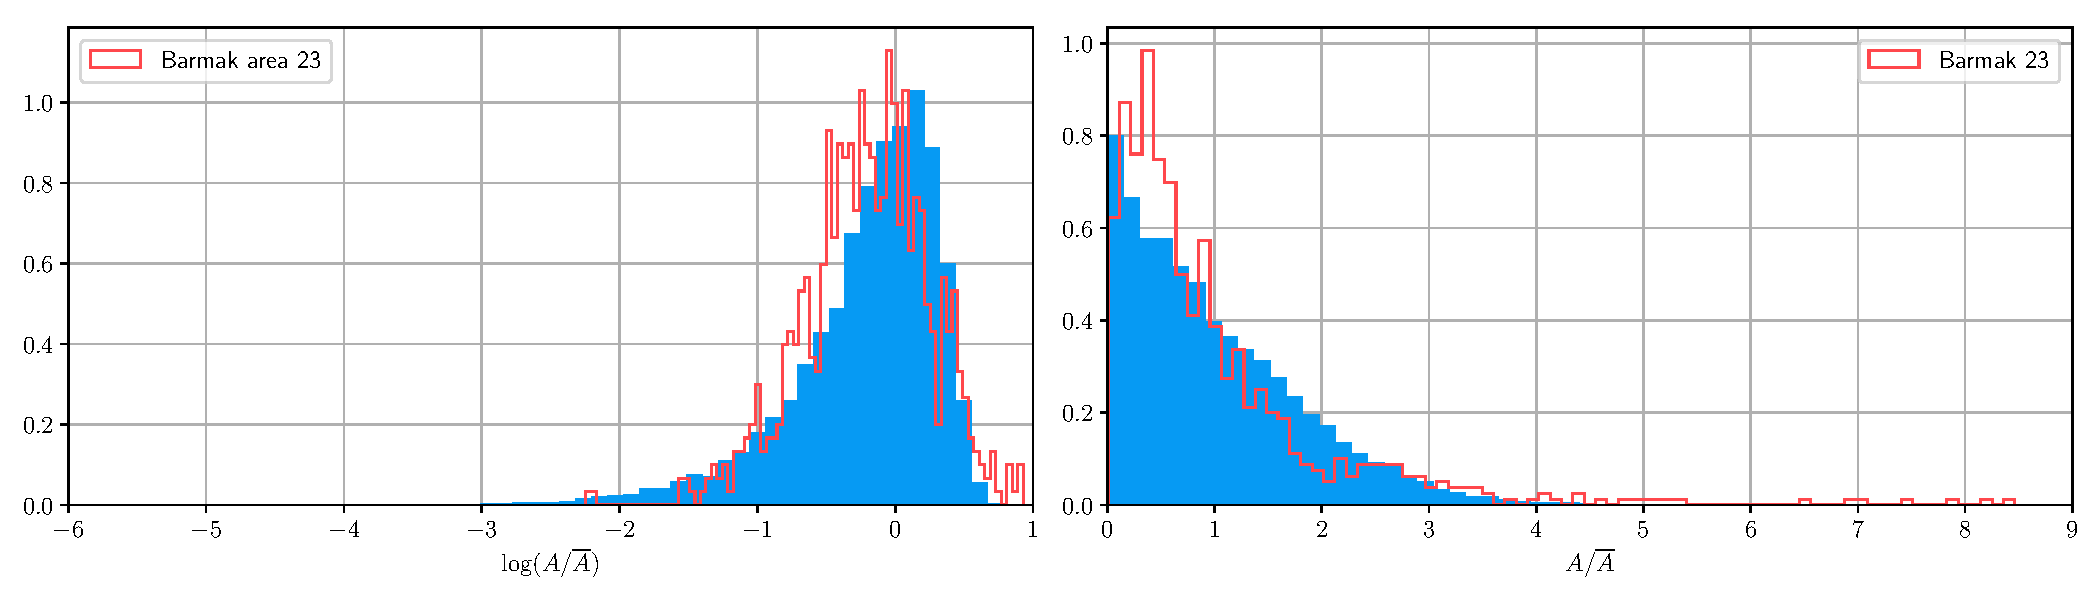
\includegraphics[scale=0.4]{figures/coupled/output_30/result__845_6_areas.pdf}
    \label{fig:coupled_1_areas}
    }\\
    \hspace{1em}
    \subfloat[Distribution of dihedral angle.]{
     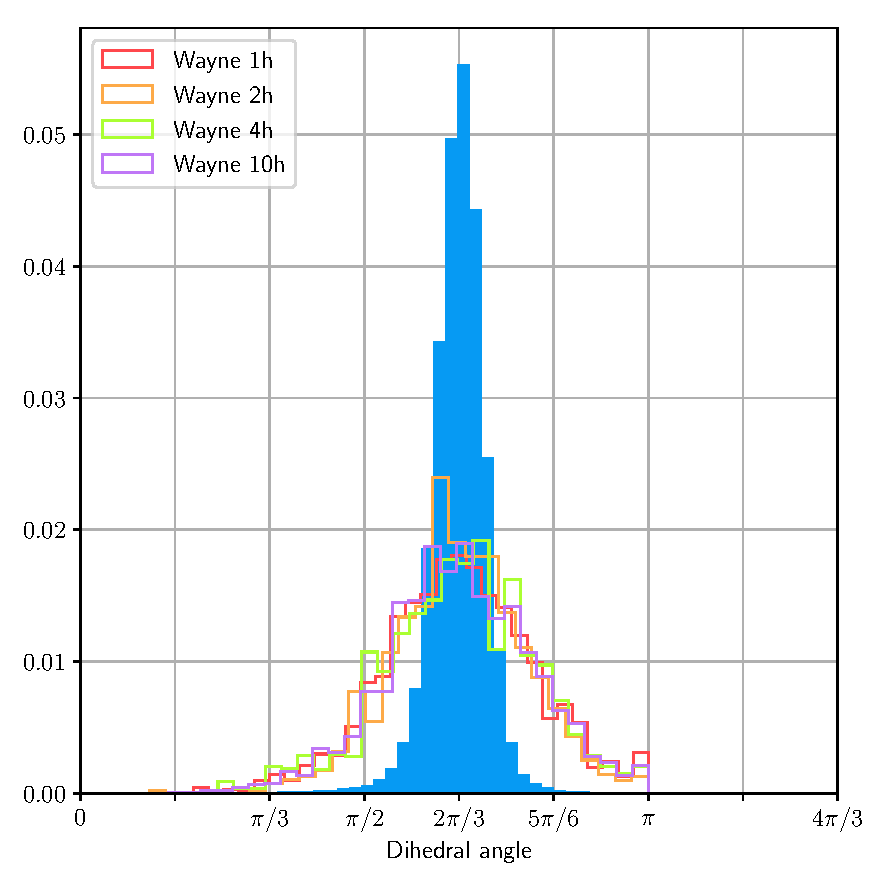
\includegraphics[scale=0.45]{figures/coupled/output_30/result__845_6_dihedral.pdf}
     \label{fig:coupled_1_dihedral}
    }
    \subfloat[GBCD]{
     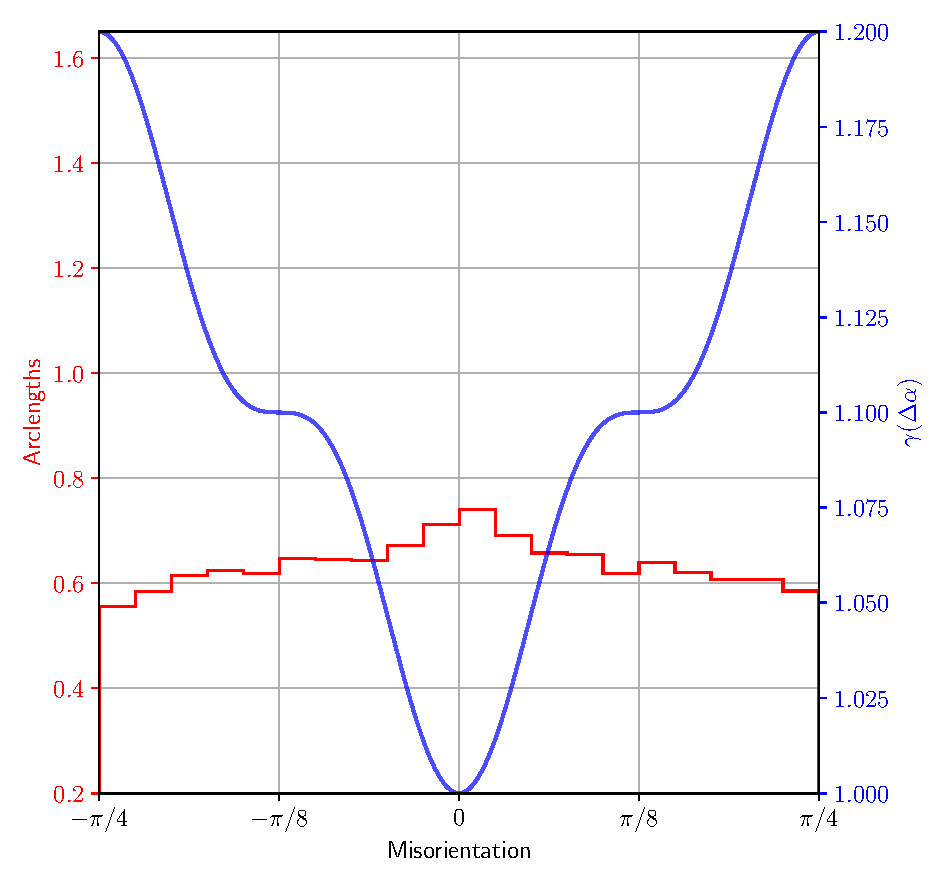
\includegraphics[scale=0.45]{figures/coupled/output_30/result__845_6_gbcd.pdf}
     \label{fig:coupled_1_gbcd}
    }\\
    \subfloat[Histogram of grains per number of sides.]{
     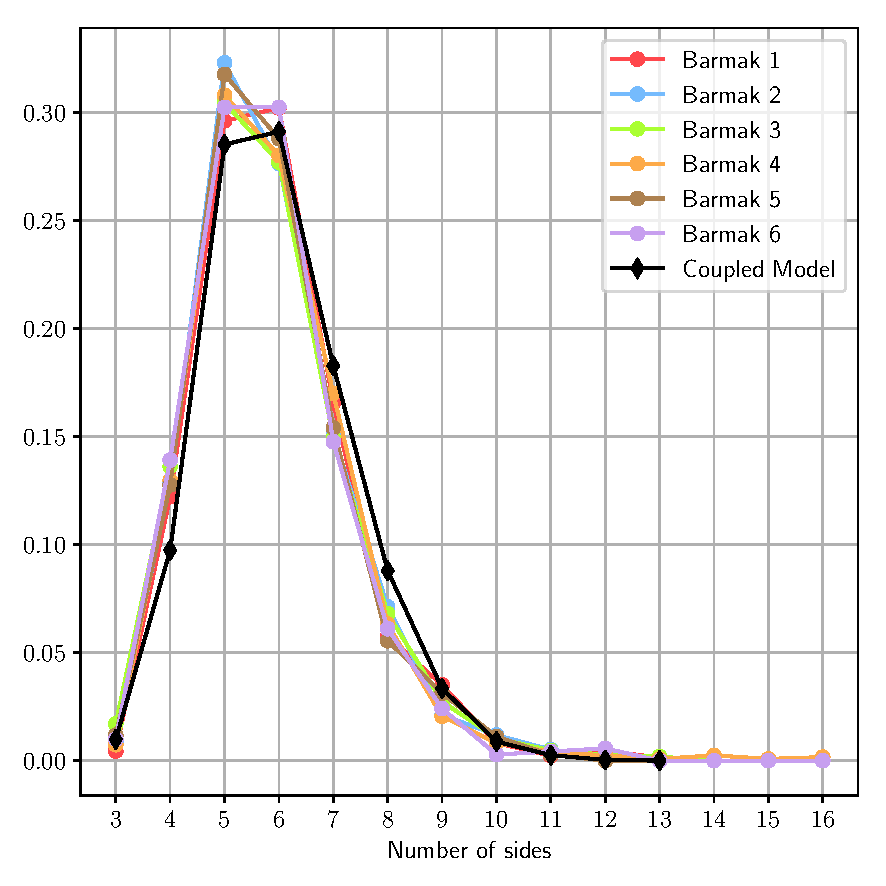
\includegraphics[scale=0.45]{figures/coupled/output_30/result__845_6_nsides.pdf}
     \label{fig:coupled_1_nsides}
    }
    \subfloat[Average number of sides of neighbors.]{
     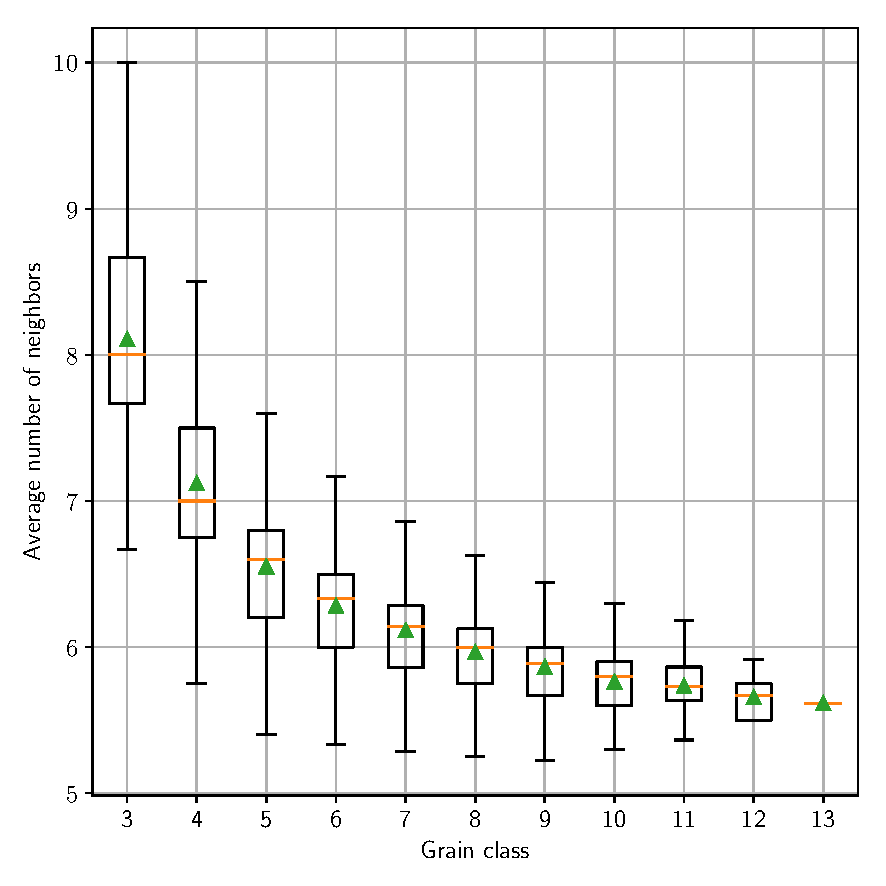
\includegraphics[scale=0.45]{figures/coupled/output_30/result__845_6_avg.pdf}
     \label{fig:coupled_1_avg}
    }
    \caption[Statistics for Coupled Model.]{Statistics for experiment with $\mu=10^{-2}, \lambda=1, \varepsilon=2\cdot10^{-1}$}
    \label{fig:coupled_1}
\end{figure}

\begin{figure}[ht]
    \centering
    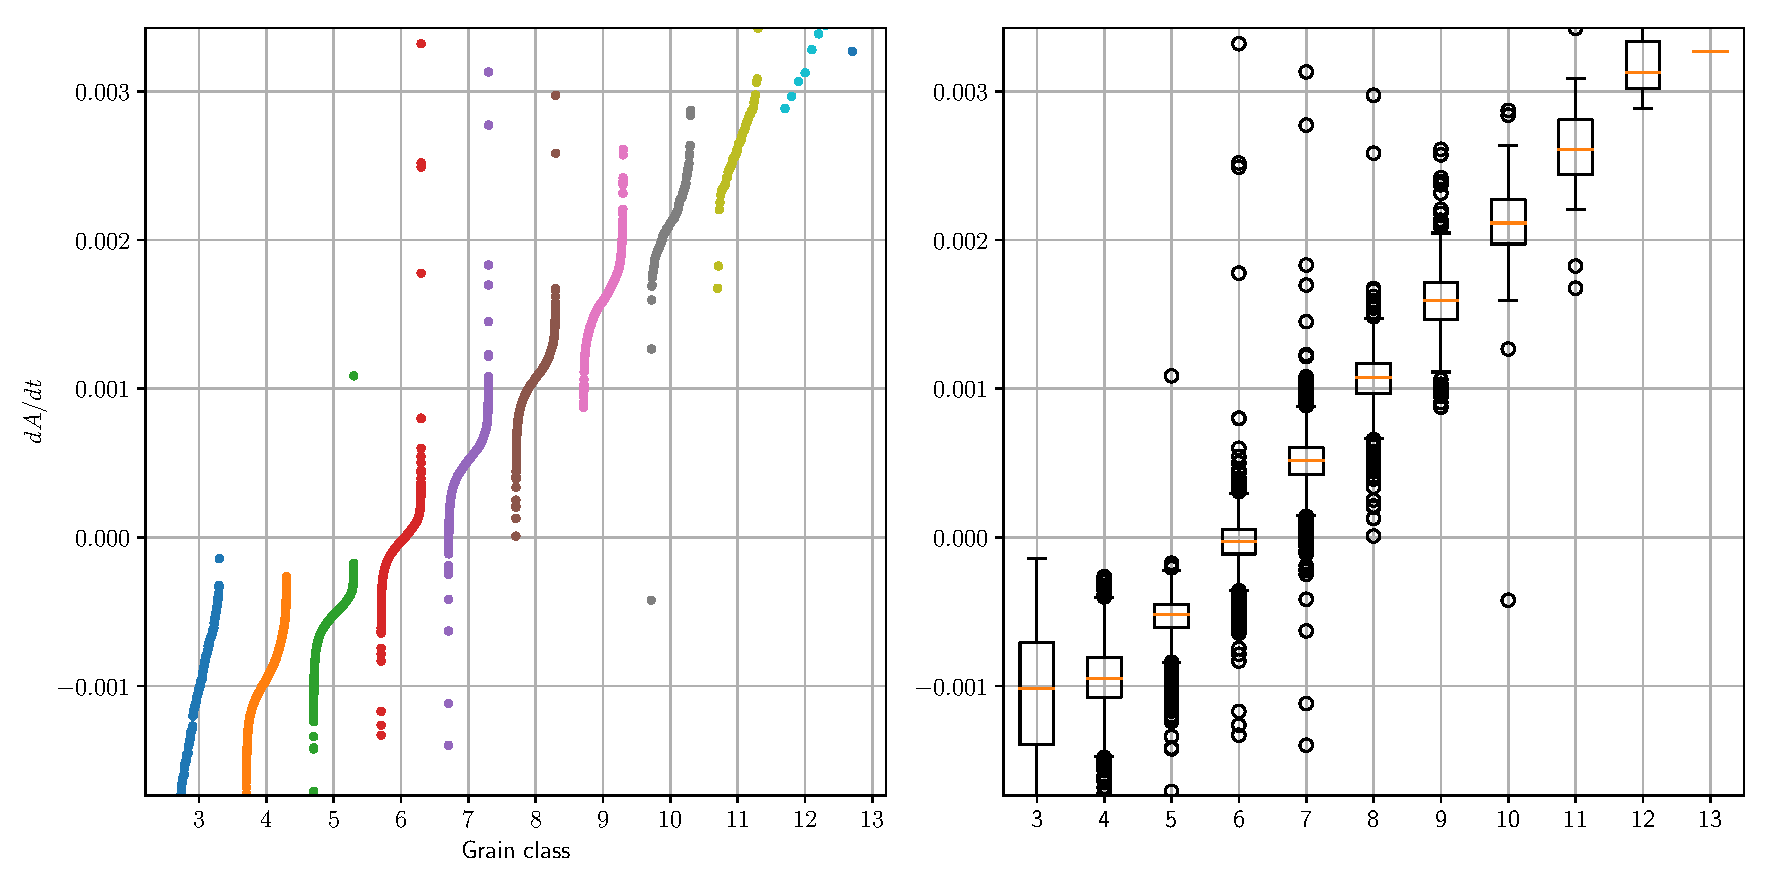
\includegraphics[scale=0.5]{figures/coupled/output_30/result__845_6_dadt.pdf}
    \caption[Area rate of change per grain class for Coupled Model.]{Area rate of change per grain class. (Left) each group of $dA/dt$ per grain class was sorted within the class and then plotted. (Right) The same groups are presented as box-plots, with the median highlighted in orange.}
    \label{fig:coupled_1_dadt}
\end{figure}
